%----------------------------------------------------------------------------------------
%    PACKAGES AND THEMES
%----------------------------------------------------------------------------------------

\documentclass[aspectratio=169,xcolor=dvipsnames]{beamer}
\usetheme{SimplePlus}
\usepackage{tikz}  % 用于绘图
\usepackage{amsmath}  % 更好的数学公式支持
\usepackage{amssymb}  % 数学符号
\usetikzlibrary{shapes, arrows, positioning, calc}  % TikZ库
\usepackage{bm}
\usepackage{xcolor}
\usetikzlibrary{decorations.pathm, patterns}
\usepackage{hyperref}
\usepackage{graphicx} % Allows including images
\usepackage{booktabs, tabularray} % Allows the use of \toprule, \midrule and \bottomrule in tables
\graphicspath{{figures/}}

%----------------------------------------------------------------------------------------
%    TITLE PAGE
%----------------------------------------------------------------------------------------
\title{曲梁结构免自锁有限元无网格法\\及其在屈曲分析中的应用}

\author{汇报人：何祖彦}

% 新增指导老师信息
\newcommand{\advisorname}{指导老师：吴俊超} % 请在此处填入指导老师的姓名

% 自定义标题页模板，包含指导老师信息和校徽
\setbeamertemplate{title page}{%
 % 在左上角添加文字
    \begin{flushleft}
        \vspace{0.5em}
        \hspace{0.5em}
        \begin{minipage}[t]{0.8\textwidth}
            \raggedright
            \usebeamerfont{institute}
            \color{DarkBlue}
            \textbf{土木工程学院2024级开题汇报}\\
        \end{minipage}
    \end{flushleft}
    \vspace{0.1em} % 调整顶部间距为logo留出空间
    
    % 在顶部添加华侨大学校徽
    \begin{center}
        
\includegraphics[width=2.5cm]{hqu2.png} % 调整校徽大小
        \vspace{0.3em}
    \end{center}
    
    \begingroup
    \centering
    % ------------------------
    \begin{beamercolorbox}[sep=1pt,center]{title}
        \usebeamerfont{title}\inserttitle\par%
        \ifx\insertsubtitle\@empty%
        \else%
        \vskip0.25em%
        {\usebeamerfont{subtitle}\usebeamercolor[fg]{subtitle}\insertsubtitle\par}%
        \fi%
    \end{beamercolorbox}%
    \vskip1em\par
    % ------------------------
    \begin{beamercolorbox}[sep=3pt,center]{author}
        \usebeamerfont{author}\insertauthor
    \end{beamercolorbox}
    % 添加指导老师信息，与作者名字保持1pt间距
    \vskip1pt
    \begin{beamercolorbox}[sep=5pt,center]{author}
        \usebeamerfont{author}\advisorname
    \end{beamercolorbox}
    \vskip0.5em
    % ------------------------
    \begin{beamercolorbox}[sep=3pt,center]{date}
        \usebeamerfont{date}\insertdate
    \end{beamercolorbox}\vskip0.5em
    % ------------------------
    {\usebeamercolor[fg]{titlegraphic}\inserttitlegraphic\par}
    \endgroup
    \vfill
}

\date{2025年12月12日} % Date, can be changed to a custom date

%----------------------------------------------------------------------------------------
%    PRESENTATION SLIDES
%----------------------------------------------------------------------------------------

\begin{document}

\begin{frame}
    % Print the title page as the first slide
    \titlepage
\end{frame}

\begin{frame}{目录}
    % Throughout your presentation, if you choose to use \section{} and \subsection{} commands, these will automatically be printed on this slide as an overview of your presentation
    \tableofcontents
\end{frame}

\section{研究背景}

% 在您的 LaTeX 文档中合适位置添加以下代码
\begin{frame}{研究背景}

\begin{center}
% 并排插入两张图片
\begin{minipage}[t]{0.48\linewidth}
    \centering
    \includegraphics[width=\linewidth]{16.jpg} \\[0.5em]
\end{minipage}
\hfill
\begin{minipage}[t]{0.48\linewidth}
    \centering
    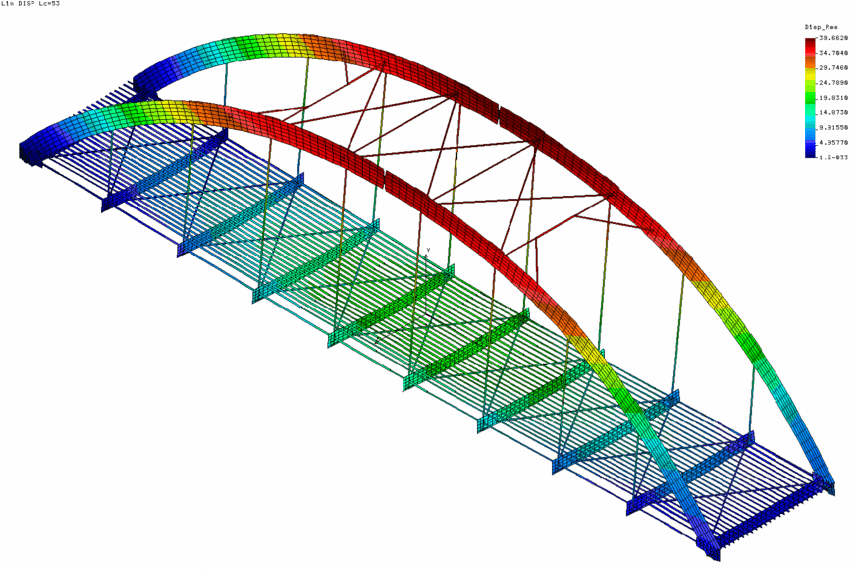
\includegraphics[width=\linewidth]{31.png} \\[0.5em]
\end{minipage}
\end{center}

\vspace{1em}

\begin{center}
\textbf{主要研究对象为考虑横向剪切应变的曲梁结构}
\end{center}

\end{frame}

\begin{frame}{研究背景}

\begin{columns}[T,totalwidth=\textwidth]
\centering
%======================== 左侧 ============================
\column{0.49\textwidth}
\centering
\textbf{几何方程与物理关系} 
\vspace{-0.5em}
{\large
\begin{align*}
\kappa &= \psi_{,s} \\[0.9em]
\epsilon &= u_{,s} - \dfrac{w}{R} \\[0.9em]
\gamma &= w_{,s} + \dfrac{u}{R} - \psi \\[1.4em]
EI &= \dfrac{Ebh^3}{12} \propto h^3 \\[0.5em]
kGA &= kG(bh) \propto h
\end{align*}
}

% ←←←←←←←←←← 不用TikZ的超強紅色爆炸框（純LaTeX） ←←←←←←←←←←
\parbox{0.96\linewidth}{
\centering
\vspace{1pt}
{\bfseries h $\to$ 0 时抗剪刚度相对弯曲刚度无限大！}
\vspace{1pt}
}

%======================== 右侧 ============================
\column{0.51\textwidth}
\centering
\textbf{屈曲理论}

\vspace{0.5em}
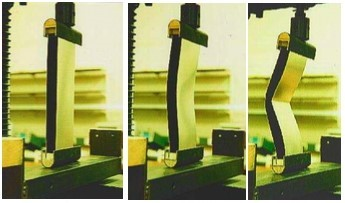
\includegraphics[width=7cm,height=6cm,keepaspectratio]{g1.jpg}

\vspace{0.1em}
\begin{block}{}
\centering
\Large $P_{\text{cr}} = \dfrac{\pi^{2} EI}{(KL)^{2}}$
\end{block}

\vspace{0.1em}
\parbox{0.94\linewidth}{
\centering
\vspace{8pt}
{\bfseries 结构在轴压下突然侧向失稳的临界载荷}\\[6pt]
\vspace{8pt}
}

\end{columns}

\end{frame}

\begin{frame}{研究背景}

\vspace{0.5em}
\begin{table}[htbp]
\centering
\small
\begin{tabular}{l|c|c}
\hline
方法 & 实验问题 & 误差(曲梁) \\
\hline
減縮積分 & 節點振盪+不穩定 & >25\% (薄梁) \\
B-bar投影 & 投影降階連續性不足 & 15\% (高階) \\
\hline
\end{tabular}
\end{table}

\vspace{0.8em}
\begin{columns}[T,totalwidth=\textwidth]
\column{0.45\textwidth}
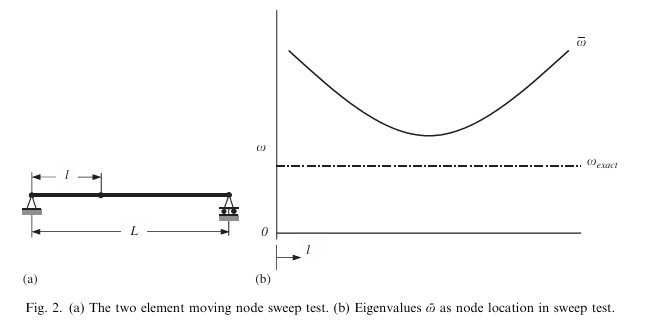
\includegraphics[width=\textwidth]{f2.png}  % Fig.2 (a/b)

\column{0.45\textwidth}
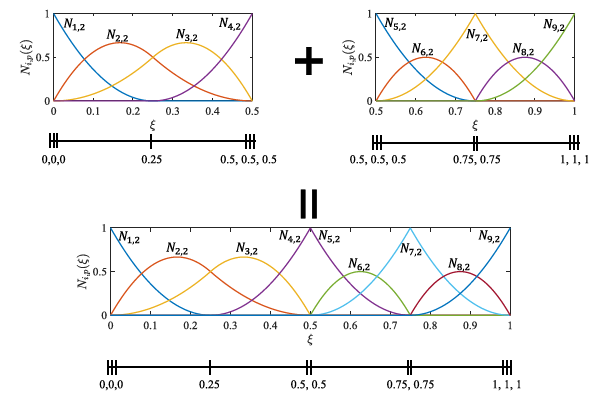
\includegraphics[width=\textwidth]{f3.png}  % NURBS基圖

\end{columns}

\vspace{6pt}

\footnotesize 来源：CMAME 2016 (Hu et al.); FEAD 2018 (Zhang et al.)。
\end{frame}

\begin{frame}{研究背景}
    \begin{columns}[T,totalwidth=\textwidth]
% 左側公式區塊（完全模仿你那張圖的排版）
\begin{minipage}{0.45\textwidth}
\textbf{混合离散分析方法}
\begin{align*}
u^{t}(s) &= \sum_{i=1}^{n_h} N_i^h(s) \, d_i \\[8pt]
w^{r}(s) &= \sum_{i=1}^{n_h} M_i^h(s) \, e_i \\[8pt]
\psi(s)   &= \sum_{i=1}^{n_h} P_i^h(s) \, \psi_i
\end{align*}
\end{minipage}

% 右側圖片區塊
\begin{minipage}{0.55\textwidth}
\centering
\begin{center}
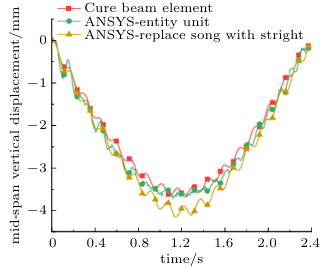
\includegraphics[width=4cm]{l1.png} % 調整圖片大小
\vspace{0.3em}
\end{center}
\end{minipage}
\end{columns}
\end{frame}

\begin{frame}{研究背景}

% 带问号的双向箭头
\begin{center}
\begin{tikzpicture}[baseline]
    % 双向箭头
    \draw[<->, line width=3.5pt, black] (0.5,0) -- (3.5,0);
    
    % 箭头上的问号
    \node[circle, draw=red, line width=1.2pt, fill=white, inner sep=2pt] at (2,0) {\textcolor{red}{\Huge\bfseries ?}};
    
    % 左侧标注
    \node[anchor=east] at (0,0) {\large\bfseries $\inf_{q \in Q} \sup_{w \in H} \frac{b(u,w,\psi)}{\|u,w\| \| \psi \|} \geq \beta > 0$};
    
    % 右侧标注
    \node[anchor=west] at (4,0) {\large\bfseries $\dim(u):\dim(w):\dim(\psi)$};

\end{tikzpicture}
\end{center}

\vspace{2em}

% 底部结论框
\begin{center}
    \begin{tikzpicture}[
        redbox/.style={draw=red, rectangle, minimum width=10cm, minimum height=1.2cm, align=center, line width=1.8pt, rounded corners=5pt, font=\large\bfseries, fill=red!5},]
        \node[redbox] (solution) {LBB稳定性条件和自由度比例之间的关系不明确};
    \end{tikzpicture}
\end{center}

\end{frame}


\section{研究方案}

\begin{frame}{研究方案}
\begin{columns}[onlytextwidth,T]
% 右侧栏：美化流程图
\begin{column}{0.5\textwidth}
    \vspace{-0.5em}
\centering
% 解决方案标题
\begin{center}
{\Large\bfseries 解決方法：}
\end{center}
% 美化流程图
\begin{tikzpicture}[
    node distance=1.5cm,
    box/.style={draw, rectangle, minimum width=3.2cm, minimum height=1cm, align=center, line width=1.2pt, rounded corners=4pt, font=\large\bfseries},
    redbox/.style={draw=red, rectangle, minimum width=4.5cm, minimum height=1.2cm, align=center, line width=1.8pt, rounded corners=5pt, font=\large\bfseries, fill=red!5},
    plus/.style={draw, circle, minimum size=1.2cm, line width=1.2pt, font=\Large\bfseries},
    arrow/.style={->, >=stealth, line width=1.2pt}
]

% 有限元框
\node[box, fill=blue!10] (fem) at (0,0) {最优约束比};

% 加号
\node[plus, fill=gray!5] (plus) at (0,-1.3) {+};

% 无网格框
\node[box, fill=green!10] (meshfree) at (0,-2.7) {新inf-sup值估计器};


% 解决方案框
\node[redbox] (solution) at (0,-4.5) {解决了的体积自锁问题};

% 连接线
\draw[arrow, red, line width=2pt, shorten >=0.1cm, shorten <=0.1cm] (0,-3.2) -- (solution);

\end{tikzpicture}
\end{column}

% 左侧栏：问题与解决方案
\begin{column}{0.5\textwidth}
\vspace{-0.5em}  % 调整顶部间距
% 问题标题
\centering
\begin{center}
{\Large\bfseries 解決问题：}
\end{center}

\begin{tikzpicture}[
    node distance=1.5cm,
    box/.style={draw, rectangle, minimum width=3.2cm, minimum height=1cm, align=center, line width=1.2pt, rounded corners=4pt, font=\large\bfseries},
    redbox/.style={draw=red, rectangle, minimum width=4.5cm, minimum height=1.2cm, align=center, line width=1.8pt, rounded corners=5pt, font=\large\bfseries, fill=red!5},
    plus/.style={draw, circle, minimum size=1.2cm, line width=1.2pt, font=\Large\bfseries},
    arrow/.style={->, >=stealth, line width=1.2pt}
]

% 有限元框
\node[box, fill=blue!10] (fem) at (0,0) {探索曲梁自锁类型分析};

% 无网格框
\node[box, fill=green!10] (meshfree) at (0,-2.3) {尋找曲梁的最优自由度比例};

% 解决方案框
\node[redbox] (solution) at (0,-4.5) {求解屈曲问题特征值};

\end{tikzpicture}

\end{column}

\end{columns}

\end{frame}

\section{研究內容}

\begin{frame}{研究内容}

曲梁弱形式：
\small
\begin{align*}
\int_0^L EA \left( \delta u_{,s} - \dfrac{\delta w}{R} \right) \left( u_{,s} - \dfrac{w}{R} \right) ds
&+ \int_0^L EI \, \delta \psi_{,s} \, \psi_{,s} \, ds 
+ \int_0^L kGA \left( \delta w_{,s} + \dfrac{\delta u}{R} - \delta \psi \right) \left( w_{,s} + \dfrac{u}{R} - \psi \right) ds \\
&= \int_0^L (p_u \delta u + p_w \delta w + m \delta \psi) ds 
+ \left[ \bar{N} \delta u + \bar{Q} \delta w + \bar{M} \delta \psi \right]_{\Gamma_N}
\end{align*}

\textbf{剪切自鎖}
\begin{align*}
\gamma = w_{,s} + \frac{u}{R} - \psi \approx 0 \quad (\gamma \neq 0)
\end{align*}

\textbf{膜自鎖}
\begin{align*}
\epsilon = u_{,s} - \frac{w}{R} \approx 0 \quad (\epsilon \neq 0)
\end{align*}

\end{frame}

\begin{frame}{研究内容}

對於剪切自鎖：
\small
\[ \beta = \inf_{\gamma^h \neq 0} \sup_{(u,w,\psi)^h} \frac{\int \gamma^h (\delta w_{,s} + \frac{\delta u}{R} - \delta \psi) \, ds}{\|\gamma^h\| \cdot \|(u,w,\psi)^h\|} \geq c > 0 \]

對於膜自鎖：
\small
\[ \beta = \inf_{\epsilon^h \neq 0} \sup_{(u,w)^h} \frac{\int \epsilon^h (\delta u_{,s} - \frac{\delta w}{R}) \, ds}{\|\epsilon^h\| \cdot \|(u,w)^h\|} \geq c > 0 \]

這些條件確保免自鎖，並應用於屈曲分析。

\end{frame}


\section{进度安排}

\begin{frame}{研究进度安排}
    \vspace{0.2cm} % 减少顶部空白
% 使用 tabularray 包创建美观的表格
\begin{tblr}{
    width = \textwidth,
    colspec = {X[1.02, l] X[2.3, l] X[0.8, c]},
    row{1} = {bg=MediumBlue!20, fg=black, font=\bfseries},
    row{2-Z} = {abovesep=5pt, belowsep=5pt},
    row{6} = {font=\normalsize},
    cell{7}{1} = {c=3}{r},
    hlines = {1pt, black},
    vlines = {},
}
\textbf{时间} & \textbf{研究内容} & \textbf{进度情况} \\

2023.7-2023.12 & 验证LBB稳定性条件与自由度比例之间的关系 & 
\raisebox{-0.2ex}{\begin{tikzpicture}[baseline=(a.base)]
    \node[circle, fill=black, inner sep=3pt] (a) {};
\end{tikzpicture}} \\

2024.1-2024.2 & 进行Timoshenko曲梁的无网格有限元混合离散分析 & 
\raisebox{-0.2ex}{\begin{tikzpicture}[baseline=(a.base)]
    \node[circle, draw=black, thick, inner sep=3pt] (a) {};
\end{tikzpicture}} \\

2024.3-2024.9 & 曲梁结构免自锁在屈曲分析中的应用 & \\

2024.10-2024.12 & 整理成果并完成论文初稿撰写 & \\

2025.1-2025.3 & 进一步修改完善论文，形成并提交论文终稿 & \\

\scalebox{2}{$\bullet$}已完成 \quad \scalebox{2}{$\circ$} 正在进行 & & \\
\end{tblr}

% 在表格和图例之间添加弹性空间
\vspace*{\fill}

% 在页面底部添加2em的固定距离
\vspace{2em}
\end{frame}

\begin{frame}
    \Huge{\centerline{\textbf{请各位老师批评指正！}}}
\end{frame}

\end{document}